\chapter{Speed of Sound in Air}

\section{Aim}
To determine the speed of sound in air by using a resonant tube

\section{Background Information}
When you are far from the source of sound, you might see the action before you hear it. For example, a flash of thunder is seen before the sound is heard. Sound travels more quickly through liquids than through gases and is fastest through solids. Communication between people involves the transfer of sound waves through air. There is a need to investigate how the sound travels in air and how its speed can be determined.

\section{Materials}
Tuning fork, resonance tube, ruler, retort stand with 2 clamps, funnel, water and rubber tube

\section{Procedure}
\begin{enumerate}
\item Set up the apparatus as shown in the figure below.
\item Record the frequency of the tuning fork.
\item Strike the tuning fork of known frequency on a rubber bung and hold it just above the open tube.
\item Adjust the length of the air column in the resonant tube by raising or lowering the rubber tube until a loud sound is heard. 
\item Measure the length from the top end of the resonant tube to the meniscus of the water and record it as $L_0$.
\item Obtain a second resonance by increasing the length of the air column in the resonance tube and measure the length of air column as $L_1$.
\end{enumerate}

\begin{figure}[h!]
\centering
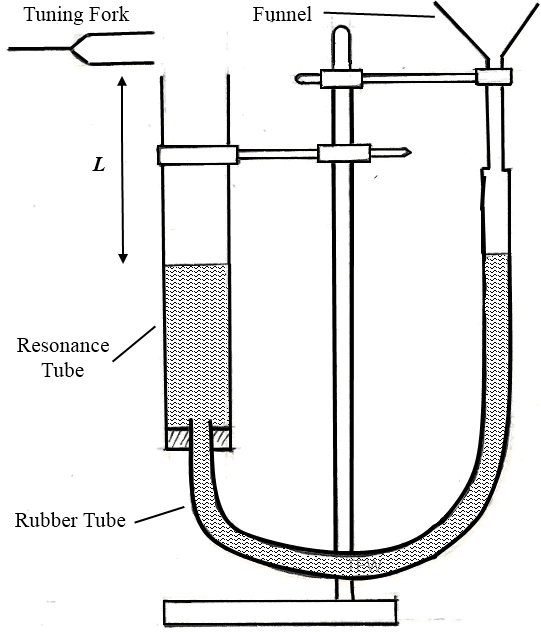
\includegraphics[width=8cm]{./img/speed-of-sound-1.png}
\caption{Speed of Sound in Air practical setup}
\label{fig:speed-of-sound-1}
\end{figure}

\section{Analysis and Interpretation}
\begin{enumerate}
\item If the first resonance is a fundamental frequency $f_0$ and the second resonant is the first overtone $f_1$, determine the wavelength of the sound wave.
\item How is the first overtone frequency related to the fundamental frequency?
\end{enumerate}

\section{Conclusion}
From the results obtained in this experiment what is the velocity of sound in air?

\section{Questions for Discussion}
\begin{enumerate}
\item Why was the tuning fork placed just above the resonant tube?
\item Why were different resonant positions found in the resonant tube?
\item Why did you strike a tuning fork with a rubber bung and not against metal?
\item What are the factors which affect the speed of sound in air?
\item Why is a wider capillary tube more suitable for carrying out this experiment than a narrow one?
\end{enumerate}

\section{Reflection and Self Assessment}
\begin{enumerate}
\item Why is it important to learn the speed of sound in different materials?
\item What was most and least interesting to you in this experiment? Explain.
\end{enumerate}